\documentclass[style=upen, size=14pt]{powerdot}
\definecolor{arany}{RGB}{255,242,0}
\hypersetup{backref=page}
\hypersetup{
    colorlinks=true,
    linkcolor=cyan,
    filecolor=magenta,      
    urlcolor=cyan}
\usepackage{graphicx}
\usepackage{amsmath}
\DeclareMathOperator*{\argmax}{argmax}
\DeclareMathOperator*{\argmin}{argmin}
\usepackage{amssymb}
\usepackage{stmaryrd}
\usepackage[latin2]{inputenc}
%\usepackage[magyar]{babel}
%\usepackage{euler}
\usepackage{tikz}
\usepackage{tikz-qtree}
\usepackage{tikz-dependency}
\usepackage{linguex}
\tikzset{every tree node/.style={align=center,anchor=north}}
%\usepackage{tabularx}
%\usepackage{threeparttable}
%\usepackage{color}
%\selectlanguage{english}
%\frenchspacing
\newcommand{\nd}{\noindent}
\newcommand{\Val}{\mathop{\mathit{Val}}}
\newcommand{\gold}{\color{arany}}
%\usepackage{tikz}
%\usepackage{tikz-qtree}
\newcommand{\qed}{\hfill\mbox{\raggedright \rule{.1in}{.1in}}}
\def\es{\mathbin\land}
\newtheorem{defi}{Definition}
\newtheorem{axioma}{Axiom}
\newtheorem{tetel}{Theorem}
\newtheorem{prop}{Proposition}
\newtheorem{lemma}{Lemma}
\begin{document}

\title{Natural Language Processing\\~~\\Lecture 2\\Linguistic Structure\\ and the
  Traditional Pipeline}
% \author{}

\date{Andr�s Simonyi, ELTE, Department of AI, 2021}

\maketitle

\section[toc=Linguistic structure]{Linguistic structure}

\begin{slide}{Representation levels}
  Natural languages are very complex sign systems, and their signs (words,
  phrases, sentences etc.) have dramatically more internal structure than
  ordinary symbols. Linguists typically distinguish at least the following four
  levels of linguistic representation in a linguistic sign:\footnote{The
    discussion of representation levels and grammars in this section closely
    follows Marcus Kracht's
    \href{https://linguistics.ucla.edu/people/Kracht/courses/ling20-fall07/ling-intro.pdf}{Intoduction to Linguistics}, which is highly recommended.}\pause
  \begin{itemize}
  \item {\gold phonological structure}: the level of individual sounds, or, in
    written language, written symbols, letters;\pause
  \item {\gold morphological structure}: the level of \emph{morphemes}, i.e.,
    minimal  meaningful linguistic units, and their organization into \emph{words};
  \end{itemize}\pause
\end{slide}

\begin{slide}[toc=]{Representation levels cont.}
  \begin{itemize}
  \item {\gold syntactic structure}: the level at which words are organized into
    well formed sentences;\pause
  \item {\gold semantic structure}: the level of \emph{meaning}, i.e., what the
    linguistic sign \emph{signifies}.\pause
  \end{itemize}
  The listed representation levels do not cover all important aspects of linguistic signs:
  \begin{itemize}\pause
  \item Semantics, at least traditionally, does not deal with the non-literal,
    context-dependent elements of meaning, which are left to {\gold pragmatics},
    while\pause
  \item the study of relationships within units larger than a sentence (paragraphs, entire
    dialogues etc.) is the subject of {\gold discourse analysis}.\pause
  \end{itemize}
\end{slide}

\begin{slide}[toc=]{Representation levels cont.}
  A simple example: a possible analysis of the representational structure of
  \emph{those purple cows}.\footnote{From
    \href{http://web.stanford.edu/group/cslipublications/cslipublications/LFG/15/abstracts/lfg10abs-jackedoff.html}{R.
      Jackendoff: The Parallel Architecture and its Lexicon}. (Morphological
    structure is covered by ``phonological structure'' in the figure.)}
  
  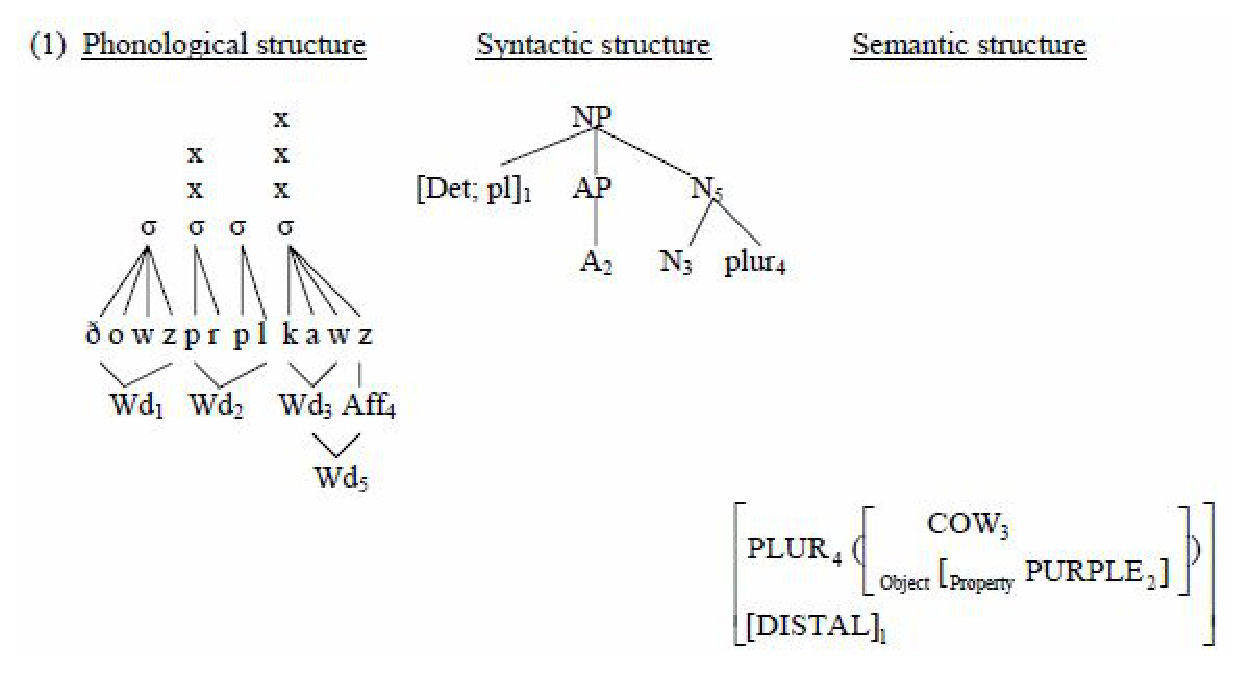
\includegraphics[width=1\textwidth]{figures/jackendoff_diagram.eps}
\end{slide}

\begin{slide}[toc=Grammars]{Grammars}
  Relying on the notion of linguistic sign (l. sign for short) we can define
  further important concepts:\pause
  \begin{itemize}
  \item A {\gold language} is a set of l. signs.\pause
  \item A {\gold grammar} is a couple consisting of a\pause
  \begin{enumerate}
  \item a set of l. signs, the language's {\gold lexicon}, and\pause
  \item a finite set of operations that map one or more l. signs to a l. sign.\pause
  \end{enumerate}
\item 
  A $\mathcal G$ grammar {\gold generates} an $\mathcal L$
  language iff $\mathcal L$ contains exactly those l. signs that are in
  $\mathcal G$'s lexicon or can be produced from $\mathcal G$'s lexicon by
  applying $\mathcal G$'s operations a finite number of times.
\end{itemize}
\end{slide}

\begin{slide}[toc=]{Grammars cont.}
  Grammatical operations are typically decomposed into phonological,
  morphological, syntactical and semantic operations working simultaneously.
  
  E.g., for a two-argument $f$ grammatical operation on linguistic signs there are
  corresponding phonological, morphological etc. operations for which
  $$
  f
  \begin{pmatrix}
          \begin{bmatrix}
           ph_1 \\           
           mor_1 \\
           syn_1 \\
           sem_1
          \end{bmatrix},
          \begin{bmatrix}
           ph_2 \\           
           mor_2 \\
           syn_2 \\
           sem_2 
         \end{bmatrix}
       \end{pmatrix}
       =
       \begin{bmatrix}
           f_{\mathrm{ph}}(ph_1, ph_2)\\           
           f_{\mathrm{mor}}(mor_1, mor_2)\\
           f_{\mathrm{syn}}(syn_1, syn_2)\\
           f_{\mathrm{sem}}(sem_1, sem_2)
         \end{bmatrix}
         $$
  for all possible arguments of $f$.
\end{slide}

\begin{slide}[toc=]{Grammars cont.}
  \emph{Terminological warning}\bigskip
  
  According to our definition, a grammar covers the phonology, morphology and
  semantics of a language in addition to its syntax. \bigskip
  
  A more limited conception of grammar is also frequently used in the literature,
  which is restricted to morphology and syntax, or syntax only. \bigskip

  Also, language is frequently defined more narrowly as a set containing only
  the \emph{sentences} (as sound or written symbol sequences) generated by the
  grammar, without their morphological, syntactic and semantic structure.
\end{slide}

\begin{slide}[toc=]{Describing grammars}
  One of the central goals of linguistics is to describe grammars generating
  (fragments of) natural languages: English grammars, Spanish grammars etc.\bigskip\pause
  
  Grammars are commonly described either
  \begin{itemize}
  \item \emph{explicitly}, by describing a lexicon and defining the operations
    that generate the elements of the language from it, or\pause
  \item \emph{implicitly}, by providing a representative set of examples from
   the language generated by the grammar, i.e., speech or text samples
    annotated with morphological, syntactic etc. analyses.\pause
  \end{itemize}
\end{slide}

\begin{slide}{Parsing and generation}
  Some grammar-related tasks are of paricular importance in NLP:\bigskip
  \pause
  
  \textbf{{\gold Parsing}}\pause
  
  \begin{itemize}
  \item Decide whether a sequence of written symbols belongs to the language
    generated by a given grammar: whether it consists of the words of the
    language, is syntactically well-formed, and meaningful.\pause
    \item Determine the morphological, syntactic and semantic structure(s)
      corresponding to a sequence of written symbols in the language
      generated by a given grammar.\pause
  \end{itemize}
\end{slide}

\begin{slide}[toc=]{Parsing and generation cont.}
  \textbf{{\gold Generation}}\bigskip\pause
  
    \begin{itemize}
    \item \emph{Unconditional}: generate elements of the grammar's language. \pause
    \item \emph{Conditional}: generate elements of the grammar's language that satisfy
      certain conditions. The conditions are often semantic, i.e., generate
      elements of the language whose semantic structure (meaning) satisfies
      certain conditions.\pause
    \end{itemize}
\end{slide}

\begin{slide}[toc=Parsing and pipeline]{Parsing and the traditional NLP pipeline}
  The task of parsing had a central place in traditional NLP because it was
  assumed that most NLP tasks can be solved by
  \begin{itemize}
  \item parsing text input and producing their representational structure
    according to specific grammar(s),\pause
  \item using the resulting analyses as features for further processing.\pause
  \end{itemize}
  The traditional NLP pipeline, accordingly, is a parsing pipeline for one or
  several grammars, in which each component produces a part of the input's
  representational structure.
\end{slide}

\begin{slide}[toc=]{Processing tasks in the traditional pipeline}
  \begin{itemize}
    \item \textit{Morphology and syntax}
    \begin{itemize}
    \item tokenization
    \item sentence splitting
    \item morphological analysis
    \item part-of-speech tagging
    \item (shallow or deep) syntactic parsing
    \end{itemize}
  \item \emph{Semantics}
    \begin{itemize}
        \item named entity recognition
        \item word sense disambiguation
        \item coreference resolution / entity linking
        \item semantic role labeling (shallow semantic parsing)\\
        \item (deep) semantic parsing
    \end{itemize}
  \end{itemize}
\end{slide}

\section{Pipeline tasks}

\begin{slide}{Tokenization}
  The task is to segment an input character sequence into small meaningful units
  called \emph{{\gold tokens}}, typically words and punctuation:\bigskip

  'This is a sentence.' $\Rightarrow$ ['This', 'is', 'a', 'sentence', '.']\bigskip

  Speaking of tokens instead of words has two important advantages:
  \begin{itemize}
  \item allows more flexibility: punctuation, emoticons etc. are not words but
    still useful units for segmentation;
  \item implies that these segments are instances of certain \emph{{\gold
        types}} that collectively constitute a \emph{{\gold vocabulary}}.
  \end{itemize}
\end{slide}

\begin{slide}[toc=]{What should count as a token?}
  The answer is task and model-dependent: e.g., for some purposes punctuation is
  irrelevant, while for others sentence boundaries and, therefore, punctuation
  are important.\bigskip

  Some influential tokenization styles nonetheless achieved ``quasi-standard''
  status. For English, the
  \href{ftp://ftp.cis.upenn.edu/pub/treebank/public_html/tokenization.html}{``Penn
    Treebank rules''} are the most common, with the following key features:
  \begin{itemize}
  \item punctuation marks are split from words and treated as separate tokens,
  \item verb contractions (like the "'s" in "she's") and clitics (like the "n't"
    in "don't") are split. 
  \end{itemize}
\end{slide}

\begin{slide}[toc=]{Type assignment and normalization}
  Tokenization can also involve determining which \emph{type} tokens belong to.
  E.g., if 'apple' and 'Apple' are instances of the same type, then our
  tokenizer standardizes or \emph{{\gold normalizes}} these to a common type
  disregarding capitalization. Typical normalization practices include
  
  \begin{itemize}
  \item ``correcting'' spelling variations and typos by tokenizing all variants
    as instances of the same type,
  \item standardizing numerical or date-type expressions
  \item and punctuation (e.g, treat "!!" as "!").
  \end{itemize}

  More radical strategies include assigning all numeric expressions or all
  words not in a predefined vocabulary to a single type.
\end{slide}

\begin{slide}[toc=]{Tokenization challenges}
  The challenges are task and approach-dependent, but also depend on the input's
  \begin{itemize}
  \item writing/alphabet (e.g., writings without spaces!),
  \item language,
  \item domain,
  \item amount of noise (e.g., number of typos).
  \end{itemize}
  For European languages and writing systems, special challenges are posed by
  \begin{itemize}
  \item abbreviations (frequently ending with a period),
  \item number expressions (possibly containing white spaces, commas and periods),
  \item "multiword expressions" (MWEs) like "New York".
  \end{itemize}
\end{slide}

\begin{slide}{Sentence splitting}
  The task is to segment the (typically pretokenized) input character sequence
  into sentences:\bigskip

  ['John', 'entered', 'the', 'room', '.', 'It', 'was', 'empty', '.'] $\Rightarrow$
  [['John', 'entered', 'the', 'room', '.'], ['It', 'was', 'empty', '.']]\bigskip

  The main challenges are
  \begin{itemize}
  \item the interdependence of sentence and token segmentation, e.g. segmenting
    fragments of the form 'xxx yyy. Zzzz' (is 'yyy.' a sentence ending or an
    abbreviation?);
  \item incorrect or lacking punctuation.
  \end{itemize}
\end{slide}

\begin{slide}[toc=Morphology]{Morphology}
 
  \emph{\gold Morphemes} are the smallest meaningful units in a language. Words can
  consist of several morphemes, e.g.\
  \emph{unbearables} = \emph{un} + \emph{bear} + \emph{able} + \emph{s}\bigskip

  Useful distinctions among morphemes:

  \begin{itemize}
  \item \emph{\gold Bound} vs \emph{{\gold free}}: free morphemes (e.g. \emph{bear})
    can stand alone as independent words, bound morphemes (e.g. \emph{-un},
    \emph{-s}) can only constitute words together with other morphemes.
  \item \emph{\gold Affixes} vs \emph{\gold roots}: roots are the main parts of the word
    with the most specific semantic content (\emph{bear} in the example), around
    which other morphemes, affixes can be placed. Most roots are free.
  \end{itemize}
\end{slide}

\begin{slide}[toc=]{Affix types}
  Affixes can be further grouped by their (typically positional) relation to other
  morphemes:\smallskip
  \begin{center}
    \small
    \begin{tabular}{ c c c }
      \hline
      Affix type & Relation  & Example \\
      \hline
      prefix & precedes & \emph{un-}, \emph{anti-} \\
      suffix & follows & \emph{-s}, \emph{-ing} \\
      infix & between & \emph{Singa{\gold bloody}pore} \\
      circumfix & around & \emph{ge...t} in German (e.g. \emph{gespielt}) \\  
      stem change & changes & Arabic \emph{kitaab} ('book')$\rightarrow$ \emph{kutub} ('books')
    \end{tabular}
  \end{center}\bigskip
  Far from being the full list, other affix types include duplication,
  tone/pitch change etc.
\end{slide}

\begin{slide}[toc=]{Affix types cont.}
  A crucial distinction is between inflectional and derivational affixes:
  \begin{itemize}
  \item \emph{\gold inflectional} affixes create new forms of the \emph{same
      word}, and can represent grammatical aspects such as person, tense etc.,
    English examples include the plural \emph{-(e)s} and the progressive \emph{-ing}.
  \item \emph{\gold derivational affixes}, on the other hand, \emph{form new
      words}, e.g., the \emph{-able} in \emph{bearable} forms an adjective from
    a verb.
  \end{itemize}
\end{slide}

\begin{slide}[toc=]{Stem and lemma}
  \begin{itemize}
  \item The \emph{\gold stem} of a word consists of the \emph{base part} of the
    word that is common in all inflected forms. Consequently, the stem is often
    not a meaningful word, e.g., the stem of \emph{produced} is \emph{produc}
    (because of \emph{producing} etc.).\footnote{The example is from Wikipedia's
      \href{https://en.wikipedia.org/wiki/Lemma_(morphology)}{Lemma entry}.}
\item A \emph{\gold lemma}, in contrast, is always a complete word, namely, the
  uninflected base form of inflected forms. Continuing the example, the lemma of
  \emph{produced} is \emph{produce}.
  \end{itemize}
\end{slide}

\begin{slide}[toc=]{Morphological analysis tasks}
  \begin{itemize}
  \item Decide whether a string is a well-formed word.
  \item \emph{\gold Stemming}: determine the stem of a word.
  \item \emph{\gold Lemmatization}: determine the lemma of a word.
  \item \emph{\gold Morphological tagging}: tag input words according to the grammatical
    information their inflections etc. express.
  \item \emph{\gold Morphological segmentation}: segment the input words into morphemes.
  \item \emph{\gold Full morphological analysis}: segment the words into morphemes and
    categorize each morpheme according to type, and grammatical information they
    convey. Often includes lemmatization too.
  \end{itemize}
\end{slide}

\begin{slide}[toc=]{Morphological analysis challenges}
  \begin{itemize}
  \item \emph{\gold Ambiguity / context dependence}: many words have multiple
    analyses that can only be disambiguated based on context, e.g.  the
    \emph{-s} in \emph{chairs}. Cf.\smallskip

    \emph{The president {\gold chairs} the meeting.}\\ 
    \emph{There were hundreds of {\gold chairs} in the room.}\smallskip 
    
  \item \emph{\gold Compounds}: many languages have compound words built from
    two or more simpler words: e.g., the German \emph{Schadenfreude} from
    \emph{Schaden} ('damage, harm') and \emph{Freude} ('joy').
  \item \emph{\gold Morphologically rich languages}: English has a relatively
    simple morphology. Other languages, e.g., Hungarian and Turkish are way more
    complex...
  \end{itemize}
\end{slide}

\begin{slide}[toc=]{Morphological analysis challenges cont.}
  Extreme Turkish example:\smallskip\\
    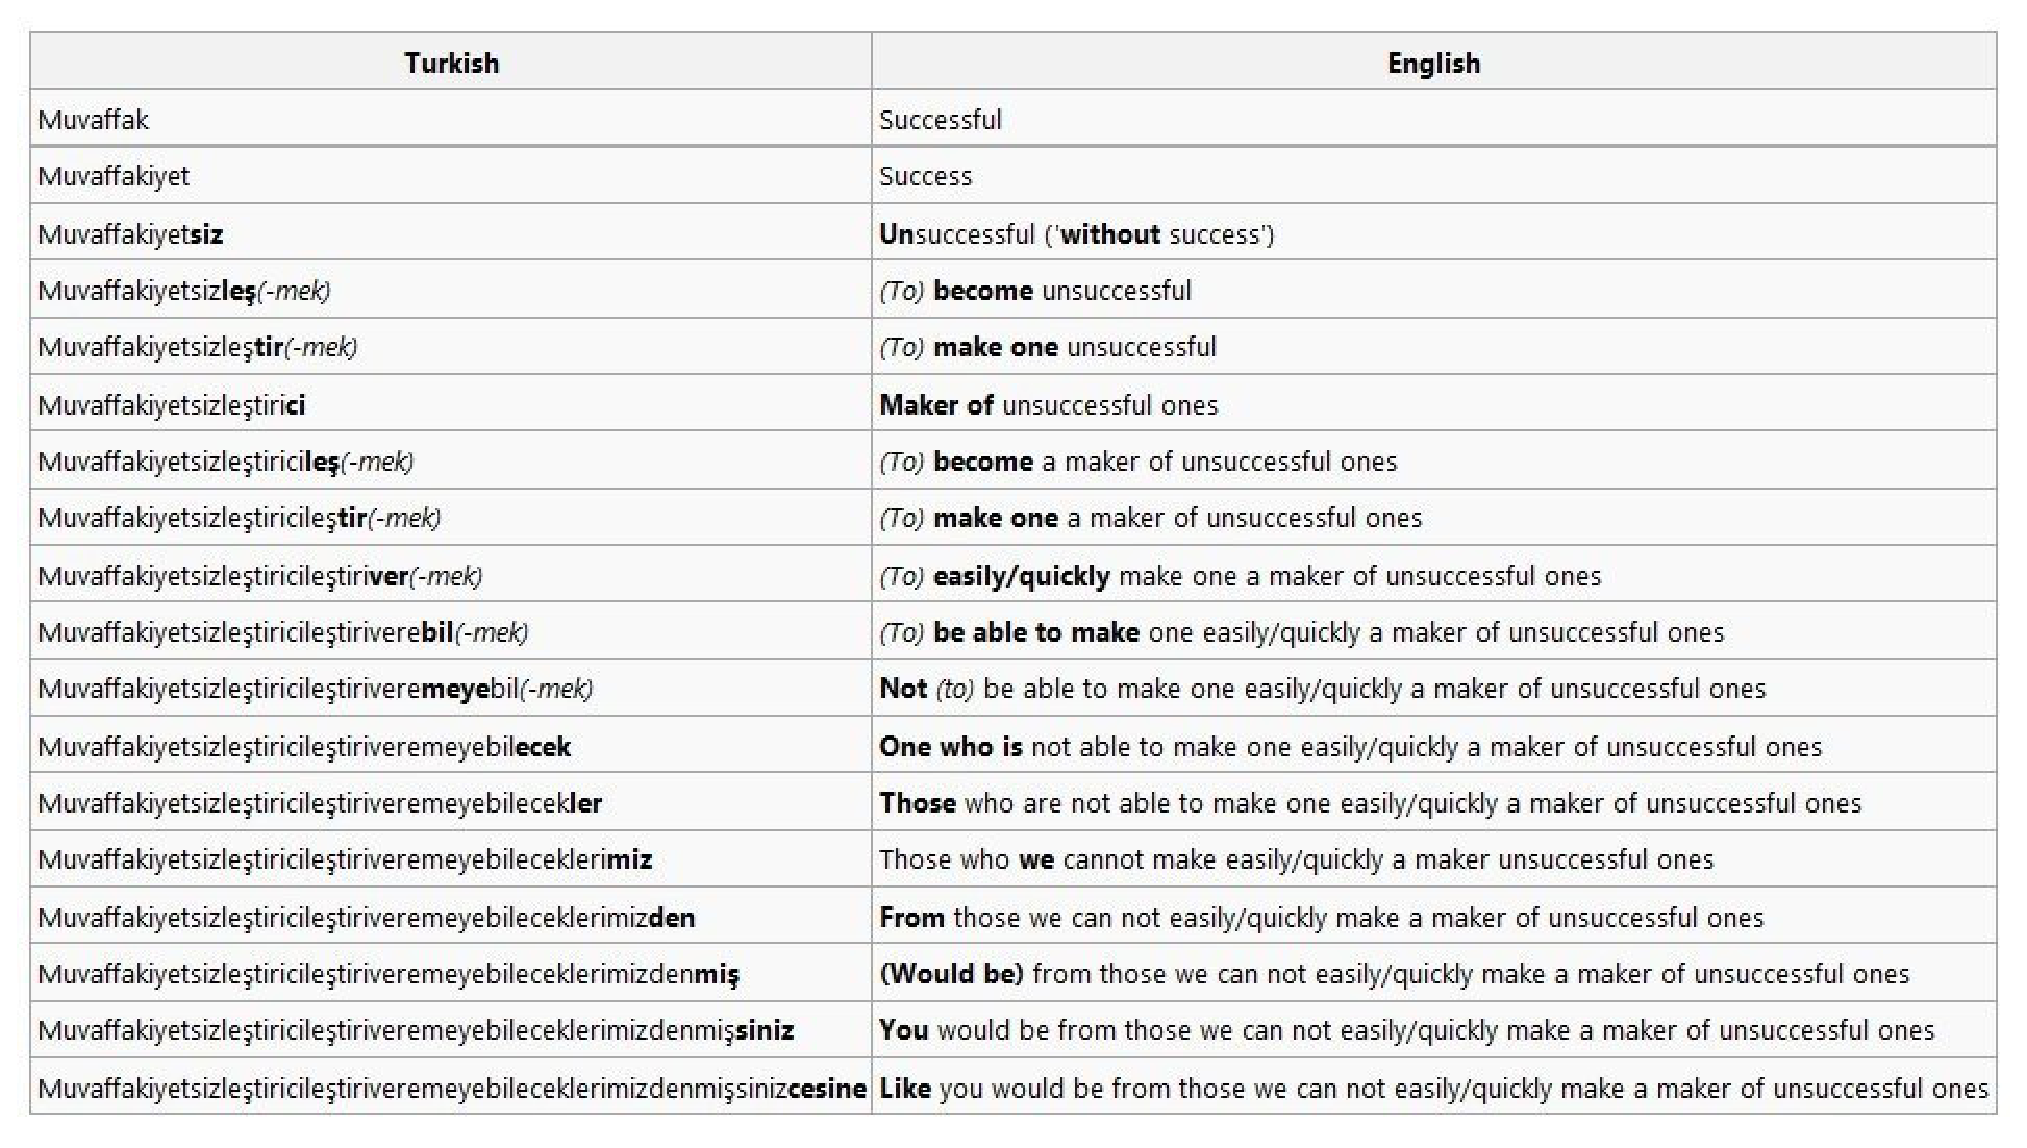
\includegraphics[width=1\textwidth]{figures/turk.eps}
\end{slide}

\begin{slide}[toc=POS tagging]{Part-of-speech tagging}
  Part-of-speech (POS for short) categories correspond to basic syntactic roles
  words can play in sentences. E.g., in the sentence\bigskip

  \emph{Peter ate the apple.}\bigskip

  \emph{Peter} and \emph{apple} are nouns, \emph{ate} is a verb and \emph{the}
  is a determiner. The POS-tagging task is to determine the POS-category of each
  word in an already tokenized (and possibly sentence-split) input text,
  e.g.,:\bigskip

  ['Peter', 'ate', 'the', 'apple', '.'] $\Rightarrow$ \\
  
  [('Peter', \textsc{'noun'}), ('ate', \textsc{'verb'}), ('the',
  \textsc{'det'}), ('apple', \textsc{'noun'}), ('.', \textsc{'punct'})]
\end{slide}

\begin{slide}[toc=]{Part-of-speech tagging cont.}
  Similarly to the morphological analysis of a word, POS-category is
  context-dependent. E.g., compare\bigskip

  \emph{John {\gold hit} the ball.}\\
  \emph{His first song was a huge {\gold hit} in Europe.}\bigskip

  The concrete list of POS categories and their delineation also depends on the
  language and specific grammatical theory used, although some are quite
  universal, e.g., the categories \textsc{noun}, \textsc{verb},
  \textsc{adjective} and \textsc{adverb} are almost always present.
\end{slide}

\begin{slide}[toc=]{Open vs. closed POS-categories}
  \begin{itemize}
  \item \emph{\gold Closed} POS categories, e.g., determiners in English, consist of
    relatively small sets of words, and these sets do not change easily: it's a
    rare phenomenon that a new determiner is added to a language.
  \item \emph{\gold Open} POS categories, like that of English verbs, contain a
    large number of words and new members are added on daily basis.
  \end{itemize}
  A related distinction is between \emph{function words} and \emph{content
    words}. Words belonging to open POS categories are typically content words:
  they have a well characterizable semantic content on their own. Closed POS
  categories contain function words not having much independent content.
\end{slide}

\begin{slide}[toc=]{POS tag sets}
  In NLP, POS categories are typically encoded with shorthands, so called POS
  tags. Several tag sets are in use even for English; a very important, language
  agnostic set was developed for the
  \href{https://universaldependencies.org/}{Universal Dependencies
    project}:\smallskip

  \begin{center}
    \small
    Open class tags\smallskip
    
    \begin{tabular}{lll}
      \hline
      Tag & Description & Examples\\
      \hline
      \textsc{adj} & adjective & big, old, green, African, first\\
      \textsc{adv} & adverb & very, well, exactly, tomorrow\\
      \textsc{intj} & interjection & psst, ouch, bravo, hello\\
      \textsc{noun} & noun & girl, cat, tree, air\\
      \textsc{propn} & proper noun & Mary, John, London, NATO\\
      \textsc{verb} & verb & run, eat, runs, ate\\
    \end{tabular}
  \end{center}
\end{slide}

\begin{slide}[toc=]{POS tag sets cont.}
  \begin{center}
    \small
    {Closed class tags}\smallskip
    
    \begin{tabular}{lll}
      \hline
      Tag & Description & Examples\\
      \hline
      ADP & adposition & in, to, during\\
      AUX & auxiliary & has, is, should, was, must\\
      CCONJ & coordinating conjunction & and, or, but\\
      DET & determiner & a, an, the, this, which, any, no\\
      NUM & numeral & 0, 1, 2, one, two\\
      PART & particle & not, 's (as in "Andrew's table")\\
      PRON & pronoun & I, myself, who\\
      SCONJ & subordinating conjunction & that, if\\
    \end{tabular}
    \smallskip
    
    \small
    {Other tags}\smallskip
    
    \begin{tabular}{lll}
      PUNCT & punctuation~~~~~~~~~~~~~~~~~~~~~~ & .  ,  ;\\
      SYM & symbol & \$,  \P, \copyright \\
      X & other & for unanalyizable elements\\
    \end{tabular}
  \end{center}
\end{slide}

\begin{slide}{Syntactic parsing}
  Syntactic theories aim to characterize ``the set of rules or principles that
  govern how words are put together to form phrases, well formed sequences of
  words.''\footnote{\href{https://linguistics.ucla.edu/people/stabler/isat.pdf}{Koopman
      et al.: An Introduction to Syntactic Analysis and Theory, p. 1.}}\bigskip

  The most important ``well formed sequences'' in this context are
  \emph{sentences}: the central goal of syntactic theories for a given language
  is to find structural rules or principles that characterize/delineate well
  formed sentences of the language in question.
\end{slide}

\begin{slide}[toc=]{Syntactic parsing cont.}
  A sentence is well formed if it has a \emph{structural description} or
  \emph{syntactic parse} which satisfies the syntactic constraints of the theory in
  question. Syntactic well formedness doesn't guarantee coherence or
  meaningfulness. To use Chomsky's famous example:
  
  \begin{quotation}
    \emph{Colorless green ideas sleep furiously.}
  \end{quotation}
  
  is syntactically well formed but nonsensical, while

  \begin{quotation}
    \emph{Furiously sleep ideas green colorless.}
  \end{quotation}

  is not even well formed.
\end{slide}

\begin{slide}[toc=]{Syntactic parsing cont.}
  \emph{\gold Constituency} (aka \emph{phrase structure}) and \emph{\gold
    dependency} based syntactic theories have been especially important for NLP.\bigskip

  A \emph{\gold constituent} is a single word or a group of consecutive words
  that form a ``natural unit''. E.g., the phrase \emph{a nice little city}
  \begin{itemize}
  \item can be put into various sentence frames like \emph{I wanted to visit
      ...}, \emph{Budapest is ...}
  \item can be an answer to a question: \emph{What did you visit?}
  \item can be substituted by pronouns: \emph{I have visited a nice little
      city.} $\Rightarrow$ \emph{I have visited it.}\footnote{See, e.g., the
      \href{https://en.wikipedia.org/wiki/Constituent_(linguistics)}{`Constituent'
        entry of Wikipedia} for further tests.}
  \end{itemize}
\end{slide}

\begin{slide}[toc=]{Constituency-based syntax}
  Constituency-based syntactic theories
  \begin{itemize}
  \item categorize constituents, and
  \item formulate rules according to which constituents can be put together to
    build larger ones, eventually building up a whole sentence.
  \end{itemize}
  The syntactic structure of a well formed sentence, is, accordingly, its
  constituency structure, e.g., for the sentence \emph{The students love their
    professors}:\bigskip
  
  [[The$_{\mathrm{D}}$ students$_{\mathrm{N}}$]$_\mathrm{NP}$[love$_\mathrm{Vt}$ [their$_{\mathrm{D}}$ professors$_\mathrm{N}$]$_\mathrm{NP}$]$_\mathrm{VP}$]$_\mathrm{S}$
  
\end{slide}

\begin{slide}[toc=]{Constituency-based syntax cont.}
  In a more transparent constituency tree form:
  \begin{center}
    \Tree[.S [.NP [.Det \textit{the} ]
               [.Noun {\textit{students}} ]]
               [.VP [.Vt {\textit{love}} ]
               [.NP [.Det \textit{their} ]
               [.Noun {\textit{professors}} ]
               ]]]  
             \end{center}
             This is the structure constituency-based parsers  output.
\end{slide}

\begin{slide}[toc=]{Dependency-based syntax}
  Dependency grammars, in contrast, treat the \emph{\gold dependency relation}
  between words as fundamental.

  The precise criteria vary from theory to theory,
  but typically a $d$ word depends on a $h$ word (equivalently, $h$ heads $d$)
  in a sentence if
  \begin{itemize}
  \item $d$ modifies the meaning of $h$, makes it more specific, e.g.
    \emph{eats} $\Rightarrow$ \emph{eats bread}, \emph{eats slowly} etc.
  \item and there is an asymmetric relationship of omissibility between them:
    $d$ can be omitted from the sentence keeping $h$ but not vice versa.
  \end{itemize}
\end{slide}

\begin{slide}[toc=]{Dependency-based syntax cont.}
  Dependency grammars impose important global constraints on the dependency
  relations within a well formed sentence, e.g., 
  
  \begin{itemize}
  \item There is exactly one independent word (the root of the sentence).
  \item All other words depend directly on exactly one word.
  \end{itemize}
  As a consequence of the constraints, the direct dependency graph of a sentence is a tree.

  Most dependency grammars work with \emph{typed direct dependencies}: there is
  finite list of direct dependency types with specific constraints on when they
  can hold.
\end{slide}

\begin{slide}[toc=]{Dependency-based syntax cont.}
  A dependency parse tree of the earlier example:
  \begin{center}
    \begin{dependency}[theme=simple, edge style={white}, label style={text=white}]
      \begin{deptext}[column sep=1em, nodes={text=white}]
        the \& students \& love \& their \& professors \\
      \end{deptext}
      \depedge{2}{1}{det}
      \depedge{3}{2}{nsubj}
      \depedge{3}{5}{dobj}
      \depedge{5}{4}{poss}
    \end{dependency}
  \end{center}
  Compared to the constituency tree, it contains fewer nodes (one per word), but
  the edges are labeled with the corresponding dependency types.
\end{slide}

\begin{slide}[toc=NER]{Named entity recognition}
  Named entity recognition (NER) is the task of finding expressions in the input
  text that are \emph{naming} entities and tagging them with the corresponding
  entity type: \bigskip

  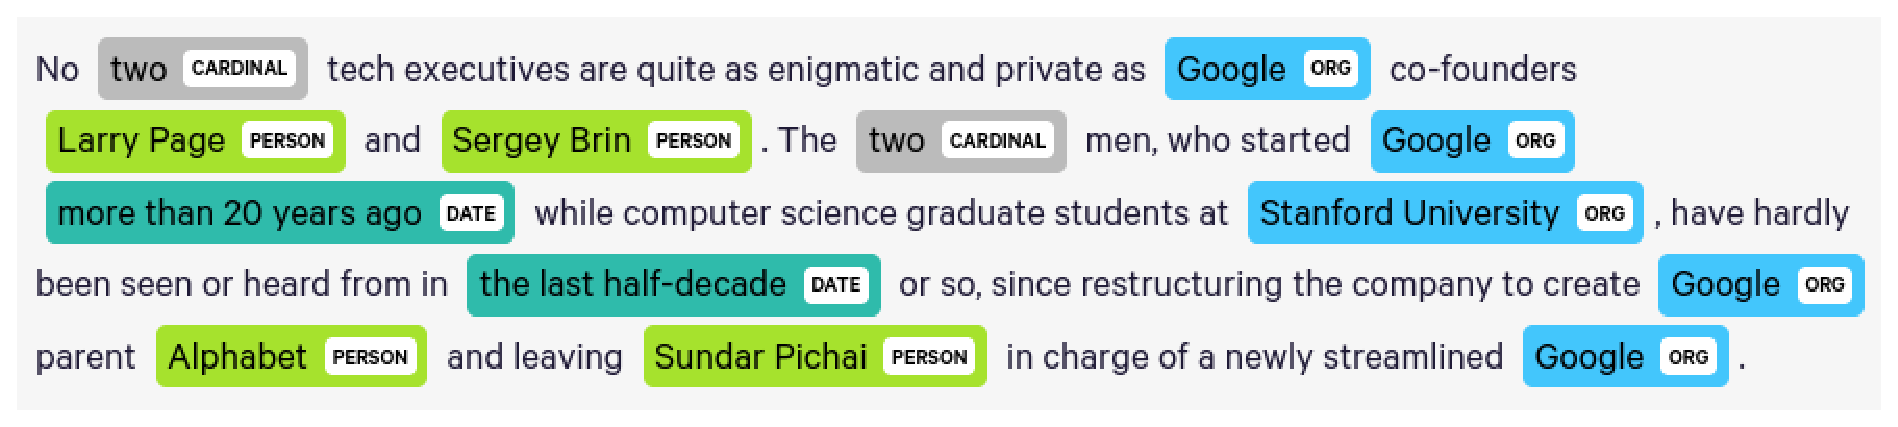
\includegraphics[width=1\textwidth]{figures/ner.eps} {\footnotesize(The figure shows
    output from spaCy's \href{https://explosion.ai/demos/displacy-ent}{NER demo
      page}.)}\bigskip

  Typically used entity types are \emph{person}, \emph{organization} and
  \emph{location}, but many NER models cover additional types such
  as \emph{date}, \emph{event}, \emph{work or art}, \emph{law} etc.
\end{slide}

\begin{slide}[toc=Coreference resolution]{Coreference resolution}
  NER determines the \emph{type} of entities that names refer to -- it doesn't
  decide whether they refer to the same or different entities. The \emph{\gold
    coreference resolution} task, in contrast, is to locate a broader range of
  referring expressions in the input including common nouns and pronouns, and
  cluster them into groups whose members all refer to the same
  entity:\footnote{The figure shows the output of the
    \href{https://spacy.io/universe/project/neuralcoref}{neuralcoref} model
    built on spaCy.}

  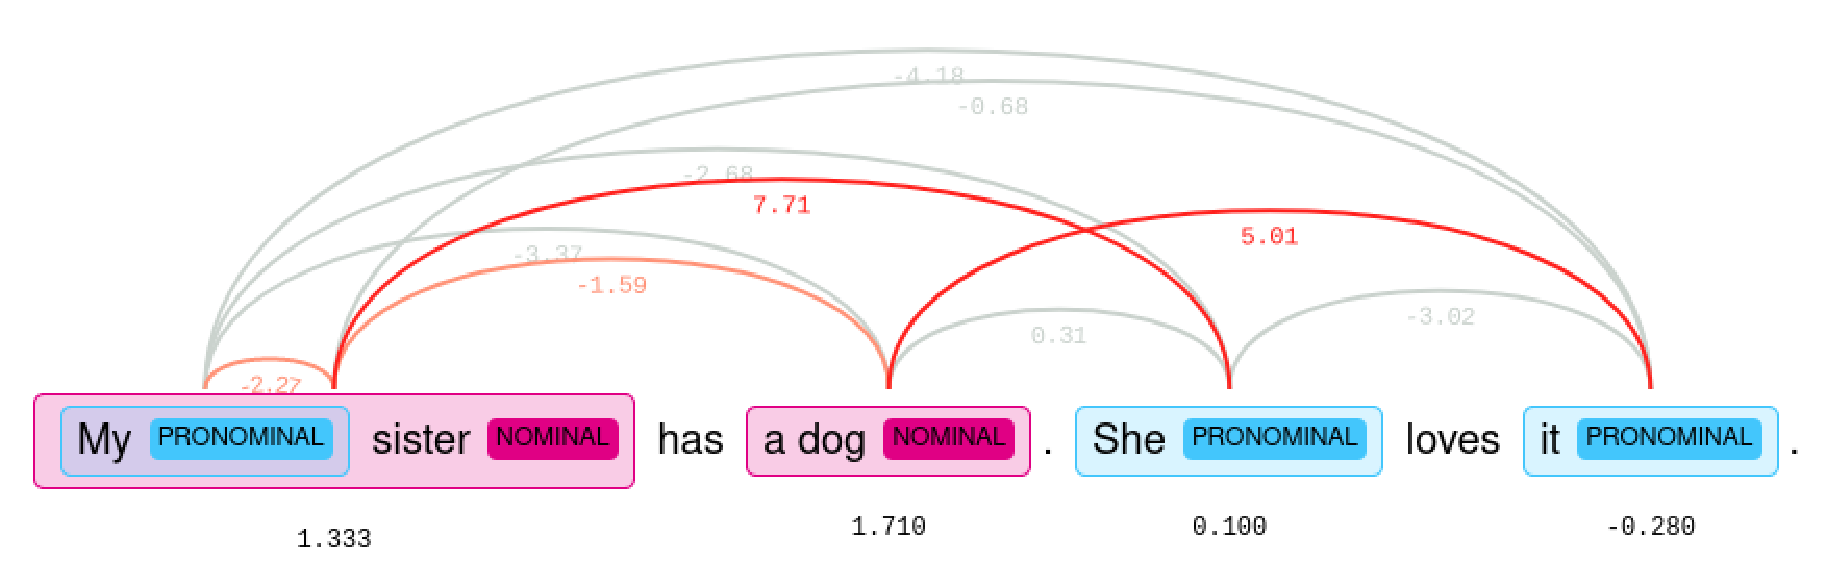
\includegraphics[width=1\textwidth]{figures/coref.eps}
\end{slide}

\begin{slide}[toc=Entity linking]{Entity linking}
  Similarly to coreference resolution, entity linking is also concerned with the
  identity of the references, but differs from it in two important respects:
  \begin{itemize}
  \item as \textsc{NER}, it is limited to name-like expressions,
  \item it determines the identity of the entities by connecting the
    names to entity records in an \emph{external} knowledge base, e.g.,
    Wikipedia:
  \begin{center}
    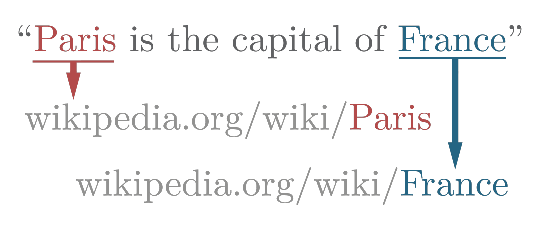
\includegraphics[width=0.6\textwidth]{figures/Entity_Linking.eps}\\
    \footnotesize{(The figure is from Wikipedia's \href{https://en.wikipedia.org/wiki/Entity_linking}{Entity Linking} entry.)}
\end{center}
\end{itemize}
\end{slide}

\begin{slide}[toc=WSD]{Word sense disambiguation}
  Word sense disambiguation also connects expressions with meanings/senses in an
  external inventory, but
  \begin{itemize}
  \item it is concerned with common nouns and other types of content words:
    verbs, adjectives and adverbs;
  \item the sense collections are typically purpose-built lexical resources --
    the quasi-standard is to use the
    \href{https://en.wikipedia.org/wiki/WordNet}{WordNet lexical database}.
  \end{itemize}
\end{slide}

\begin{slide}[toc=]{Word sense disambiguation cont.}
  For instance, a WordNet-based WSD system should disambiguate the \emph{mouse}
  noun in the sentence\bigskip

  \emph{The scroll wheel in my mouse has stopped working.}\bigskip

  to the WordNet sense\bigskip 

  \textsc{Mouse}\#4: `a hand-operated electronic device
  that controls the coordinates of a cursor [...]'. Other possibilities in WordNet:
  \begin{itemize}
  \item \textsc{Mouse}\#1: `any of numerous small rodents [...]'
  \item \textsc{Mouse}\#2: `a swollen bruise [...]'
  \item \textsc{Mouse}\#3: `person who is quiet or timid [...]'
  \end{itemize}
  
\end{slide}


\begin{slide}[toc=Semantic role labeling]{Semantic role labeling}
  Semantic role labeling (SRL) is the task of identifying \emph{\gold predicate}
  and \emph{\gold argument} expressions in the input text, determining which
  argument belongs to which predicate, and what is their relationship. In this
  context,
  \begin{itemize}
  \item \emph{\gold predicates} are expressions referring to events/situations (e.g., verbs
    referring to actions),
  \item while \emph{\gold arguments} refer to the \emph{participants} of these
    events/situations,
  \item and the \emph{\gold role labeling} part of the task is to determine what
    kind or role the participants corresponding to the arguments play in the
    situations referred to by the predicates.
\end{itemize}
\end{slide}

\begin{slide}[toc=]{Semantic role labeling cont.}
  A relatively simple example using the
  \href{https://cogcomp.seas.upenn.edu/page/demo_view/srl}{ SLR demo} of the U.
  Penn. Cognitive Computation Group:\bigskip
  
  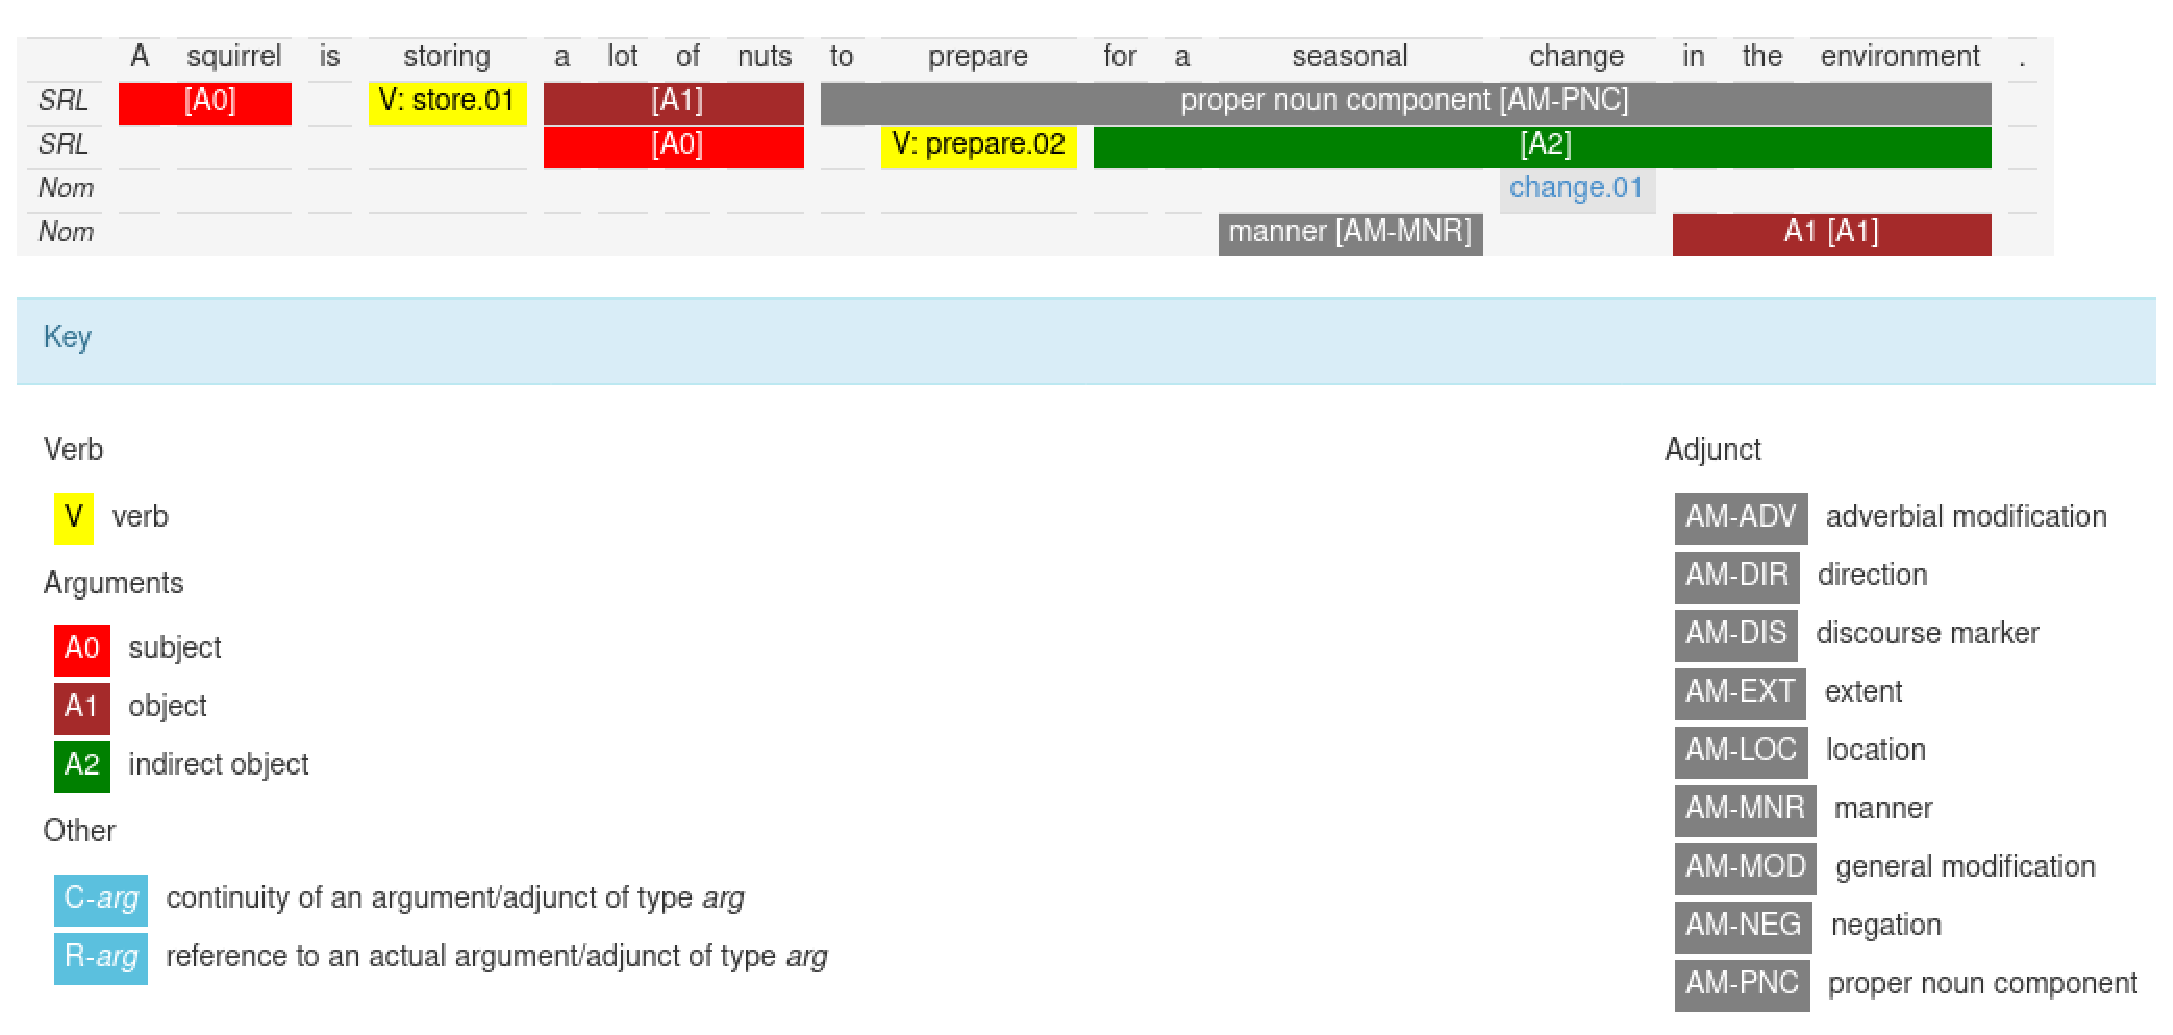
\includegraphics[width=1\textwidth]{figures/slr.eps}
\end{slide}

\begin{slide}[toc=Semantic parsing]{Semantic parsing}
  This is the the task of full or deep semantic parsing, which covers not
  ``only'' coreference resolution, WSD and predicate-argument structure, but
  aims at providing a complete formal \emph{semantic representation}, which is
  \begin{itemize}
  \item a formal structure representing the meaning of the input text,
  \item represents literal meaning,
  \item disambiguated (as far as possible),
  \item canonical (as far as possible) in the sense that a text meaning has a
    unique representation,
  \item there are efficient algorithms to determine their logical and semantic
    relationship to other semantic and knowledge representations.
  \end{itemize}
\end{slide}

\begin{slide}[toc=]{Semantic parsing cont.}
  A first-order logic based semantic representation of the sentence \emph{Thetis
    loves a mortal}:\footnote{From the
    \href{https://plato.stanford.edu/entries/computational-linguistics/}{Computational
      Linguistics entry} of the Stanford Encyclopedia of Philosophy.}\bigskip

  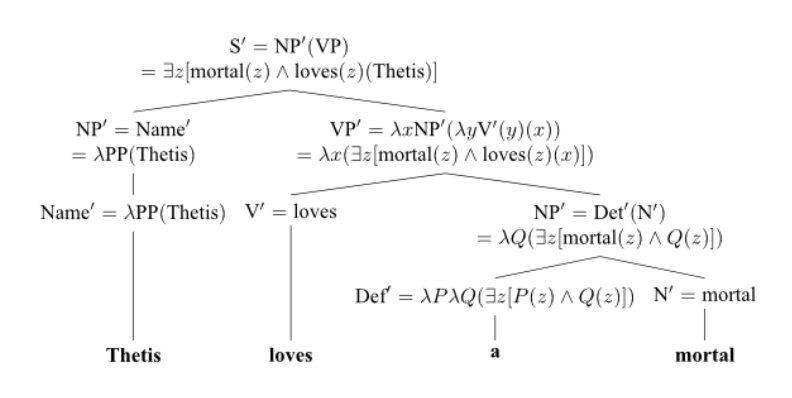
\includegraphics[width=1\textwidth]{figures/semrep.eps}.
\end{slide}

\end{document}



%%% Local Variables:
%%% mode: latex
%%% TeX-master: t
%%% End:

% LocalWords:  Tokenization
